\begin{mdframed}[style=warning]
	\textbf{Conceptos}
		\begin{enumerate}
			\item ¿Qué predice la ley de gas ideal acerca del volumen de una muestra de gas a cero absoluto? ¿Por qué esta predicción es incorrecta?
			\item El péndulo de cierto reloj se fabrica de latón. Cuando la temperatura aumenta, ¿el periodo del reloj aumenta, disminuye o permanece igual? Explique.
		\end{enumerate}
\end{mdframed}



















\begin{mdframed}[style=warning]
	\begin{ejercicio}
		Si se cierra un pistón conectado a un resorte con constante de $2\times 10^3 N/m$. Con el resorte relajado, el cilindro está lleno con $5L$ de gas a una presión de $1atm$ y una temperatura de $20^o C$. $a)$ Si el pistón tiene un área de sección transversal de $0.010m^2$ y masa despresiable, ¿a qué altura subirá cuando la temperatura se eleve a $250^o C$? $b)$ ¿Cuál es la presión del gas a $250^oC$?
	\end{ejercicio}
\end{mdframed}


























\begin{mdframed}[style=warning]
	\begin{ejercicio}
		Un reloj con un péndulo de latón tiene un periodo de $1s$ a $20^o C$. Si la temperatura aumenta a $30^o C$, $a)$ ¿en cuánto cambia el periodo y $b)$ cuánto tiempo gana o pierde el reloj en una semana?
	\end{ejercicio}
\end{mdframed}


















\begin{mdframed}[style=warning]
	\begin{ejercicio}
		Un líquido con un coeficiente de expansión volumétrica $\beta$ justo llena un atraz esférico de volumen $V_i$ a una temperatura de $T_i$. El matraz está fabricado de un material con un coeficiente de expansión lineal promedio $\alpha$. El líquido es libre de expandirse en un capilar abierto de área $A$ que se proyecta desde lo alto de la esfera. $a)$ Si supone que la temperatura aumenta en $\Delta T$, demuestre que el líquido se eleva en el capilar en la cantidad $\Delta h$ conocida por la ecuación $\Delta h = (V-i/A)(\beta - 3\alpha) \Delta T$. $b)$ Para un sistema típico, como un termómetro de mercurio, ¿por qué es una buena aproximación ignorar la expansión del bulbo?
		\begin{figure}[H]
			\centering
			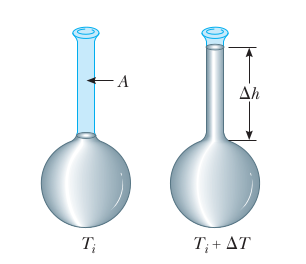
\includegraphics[scale=0.5]{./img/bulbo.png}
			\caption{Ejercicio 3}
			\label{bulbo}
		\end{figure}
	\end{ejercicio}
\end{mdframed}






















%%%